%----------------------------------------------------------------------------------------
% Preambulo y Configuración
%----------------------------------------------------------------------------------------

\documentclass[
    11pt,
    spanish,
    singlespacing,
    parskip,
    headsepline,
    bookmarks=true,
    unicode=true,
    pdftoolbar=true,
    pdfmenubar=true,
    pdffitwindow=false,
    colorlinks=true,
    linkcolor=blue,
    citecolor=blue,
    urlcolor=blue
]{MastersDoctoralThesis}

\usepackage[utf8]{inputenc} % Codificación de entrada UTF-8
\usepackage[T1]{fontenc}    % Codificación de salida para caracteres especiales
\usepackage{graphicx}       % Manejo de gráficos
\usepackage{eso-pic}        % Permite agregar fondos
\usepackage{array}
\newcolumntype{L}[1]{>{\raggedright\arraybackslash}p{#1}}
\usepackage{hyperref}       % Manejo de hipervínculos y marcadores
\usepackage{booktabs}
\usepackage{float}
\usepackage{lscape}
\usepackage{multirow} % en el preámbulo

% Redefinición de caracteres problemáticos en marcadores
\hypersetup{
    pdftitle={Título del Documento},
    pdfauthor={Autor del Documento},
    pdfkeywords={Sistemas Embebidos, Internet de las Cosas, Inteligencia Artificial},
    pdfstartview={FitH},
    unicode=true,
    colorlinks=true,
    linkcolor=blue,
    citecolor=blue,
    urlcolor=blue
}

\pdfstringdefDisableCommands{%
  \def\texttt#1{#1}%
  \def\textbf#1{#1}%
  \def\textit#1{#1}%
  \def\"{\"}%
  \def\~{~}%
  \def\'{'}%
  \def\^{}%
  \def\textunderscore{\_} % Manejo del subrayado en marcadores
}


% Definir comandos requeridos por la clase
\newcommand{\degreename}{Maestría en Ciencias} % Cambia según tu título
\newcommand{\univname}{Universidad Nacional de Ejemplo} % Cambia según tu universidad
\newcommand{\keywordnames}{Palabras clave:}
%----------------------------------------------------------------------------------------
% Documento Principal
%----------------------------------------------------------------------------------------

\begin{document}

% Configuración de la portada
\posgrado{Carrera / Maestría}
\keywords{Sistemas Embebidos, Internet de las Cosas, Inteligencia Artificial}

% Incluir la portada desde un archivo separado
\include{portada}

% Configuración del contenido preliminar
\frontmatter % Usar numeración romana para las páginas preliminares
\pagestyle{plain} % Estilo de encabezado simple

%----------------------------------------------------------------------------------------
% Resumen
%----------------------------------------------------------------------------------------

\begin{abstract}
\addchaptertocentry{\abstractname} % Agregar resumen al índice
En la presente memoria se describe el desarrollo de un sistema de inteligencia artificial enfocado en la predicción de tareas de imaginación motriz usando señales de electroencefalografía. Este trabajo busca dejar una base técnica para el desarrollo de sistemas de interacción cerebro-computador en imaginación motriz para predecir la intención de movimiento en usuarios.                                                     

Para su implementación fueron necesarios los conocimientos adquiridos en la especialización incluidos procesamiento y análisis de datos, aprendizaje automático, redes neuronales y operaciones.
\end{abstract}

%----------------------------------------------------------------------------------------
% Agradecimientos
%----------------------------------------------------------------------------------------
\begin{acknowledgements}
\vspace{1.5cm}
A mi familia, por ser el motor que impulsa mis sueños.

Por estar presente en cada paso, por creer en mí incluso cuando el camino parecía incierto y por recordarme siempre que detrás de cada meta existe una razón para seguir adelante.

Cada logro lleva un poco de ustedes: su amor, su paciencia, sus palabras de ánimo y todos esos pequeños sacrificios que muchas veces pasan desapercibidos, pero que hacen posible llegar más lejos.

Este proyecto, este sueño y todo lo que está por venir también les pertenece.

Gracias por ser mi inspiración, mi fuerza y mi hogar.
.
\end{acknowledgements}

%----------------------------------------------------------------------------------------
% Índice
%----------------------------------------------------------------------------------------

\tableofcontents
\listoffigures
\listoftables

%----------------------------------------------------------------------------------------
% Dedicatoria
%----------------------------------------------------------------------------------------

\dedicatory{\textbf{Dedicado a... [OPCIONAL]}}

%----------------------------------------------------------------------------------------
% Capítulos
%----------------------------------------------------------------------------------------

\mainmatter % Iniciar numeración numérica para el contenido principal
\pagestyle{thesis} % Estilo de encabezado de tesis

% Incluir capítulos desde archivos separados
% Chapter 1

\chapter{Introducción general} % Main chapter title

\label{Chapter1} % For referencing the chapter elsewhere, use \ref{Chapter1} 
\label{IntroGeneral}

En este capítulo se presentan los fundamentos de las tecnologías de interfaz cerebro-computador y se describe el estado actual de la investigación en el área. Asimismo, se exponen la motivación, los objetivos y el alcance definidos para el desarrollo del proyecto.

%----------------------------------------------------------------------------------------

% Define some commands to keep the formatting separated from the content 
\newcommand{\keyword}[1]{\textbf{#1}}
\newcommand{\tabhead}[1]{\textbf{#1}}
\newcommand{\code}[1]{\texttt{#1}}
\newcommand{\file}[1]{\texttt{\bfseries#1}}
\newcommand{\option}[1]{\texttt{\itshape#1}}
\newcommand{\grados}{$^{\circ}$}

%----------------------------------------------------------------------------------------

%\section{Introducción}

%----------------------------------------------------------------------------------------
\section{Interfaces cerebro-computador}

Las interfaces cerebro-computador o \textit{BCI} (del inglés, \textit{Brain-Computer Interface}) se definen como sistemas que establecen una vía de comunicación directa entre el cerebro humano y un dispositivo externo \cite{wolpaw2002bci}. Estos sistemas permitieron la traducción de patrones de actividad cerebral en comandos de control sin la intervención de las vías periféricas neuromusculares tradicionales.

El funcionamiento de una \textit{BCI} se fundamentó en la adquisición de señales bioeléctricas, su procesamiento digital y la posterior ejecución de acciones en un entorno computacional o físico. En el desarrollo de este proyecto, se consideraron las señales electroencefalográficas o \textit{EEG} (del inglés, \textit{electroencephalogram}) debido a su naturaleza no invasiva y su capacidad para registrar la intención motriz del usuario en tiempo real. La integración de estos dispositivos con servicios en la nube facilita el procesamiento de grandes volúmenes de datos, optimizando la capacidad de respuesta del los sistemas ante tareas de imaginación motriz.


\subsection{Arquitectura funcional de un sistema BCI}

El modelo operativo de una \textit{BCI} inicia con una cadena de procesamiento compuesta por etapas secuenciales. En la fase inicial, se realiza la adquisición de señales mediante sensores electroencefalográficos colocados sobre el cuero cabelludo. Luego, los datos crudos se somenten a procesos de pre-procesamiento para la eliminación de artefactos, tales como parpadeos o movimientos musculares, mediante el uso de filtros digitales.
Posteriormente, se realiza la extracción de características que permite identificar los componentes relevantes de la señal asociados a la intención del usuario. Finalmente, se implementan algoritmos de clasificación para traducir dichas características en comandos de control.


\subsubsection{Imaginación motriz y ritmos sensorimotores}

La imaginación motriz se define como el proceso cognitivo en el cual un individuo simula mentalmente una acción motora sin ejecutar un movimiento físico real \cite{pfurtscheller2001motor}. Este fenómeno produce cambios detectables en los ritmos sensoriales de la corteza cerebral, específicamente en las bandas de frecuencia mu (8-13 Hz) y beta (13-30 Hz).

\subsection{Dispositivos de adquisición de señales EEG}

La captura de la actividad eléctrica cerebral se realiza habitualmente mediante sistemas de \textit{EEG}, los cuales se clasifican según su movilidad y el tipo de sensores empleados. En el ámbito de la investigación, se destacan dispositivos de grado médico y equipos portátiles diseñados para aplicaciones fuera del entorno clínico \cite{casson2010wearable}.

Aunque en este proyecto se utilizó un conjunto de datos o dataset previamente registrado, la comprensión de estos dispositivos resultó pertinente para el análisis de la calidad de la señal.

%----------------------------------------------------------------------------------------

\section{Estado del arte}

La presente revisión del estado del arte tiene como objetivo identificar las metodologías dominantes en la clasificación de tareas de imaginación motriz mediante \textit{EEG}. En los últimos años, el estudio de las BCI ha cobrado relevancia debido a la convergencia entre la neurociencia computacional y el aprendizaje profundo, lo cual permite aprender directamente de las señales crudas,
sin depender de métodos tradicionales de extracción de características como el patrón especial común o \textit{CSP} (del inglés, \textit{Common Spatial Pattern})\cite{schirrmeister2017deep}.

Las redes neuronales convolucionales o \textit{CNN} (del ingles, \textit{Convolutional Neural Network}) constituyen una de las aproximaciones más utilizadas. Estas redes capturan patrones espaciales en las señales \textit{EEG} y han demostrado un buen desempeño en la clasificación de tareas de imaginación motriz. Modelos como EEGNet introducen arquitecturas compactas que logran buenos resultados incluso con pocos datos de entrenamiento \cite{lawhern2018eegnet}.

Por otra parte, las redes recurrentes, especialmente las de memoria a corto y largo plazo o \textit{LSTM} (del inglés, \textit{Long Short-Term Memory}), permiten modelar la dinámica temporal de las señales \textit{EEG}. Estas arquitecturas capturan dependencias en el tiempo que resultan clave para identificar patrones asociados a la imaginación de movimiento. Estudios recientes reportan que modelos basados en LSTM alcanzan desempeños superiores frente a métodos tradicionales \cite{roy2019deep}.

Asimismo, las arquitecturas híbridas que combinan \textit{CNN} y \textit{LSTM} han ganado relevancia. Estas combinaciones permiten integrar información espacial y temporal en un mismo modelo. Investigaciones muestran que este enfoque mejora la capacidad de generalización y aumenta la precisión en comparación con modelos individuales  \cite{bashivan2015learning,roy2019deep}.

En los trabajos más recientes, se han propuesto variantes más eficientes como redes convolucionales ligeras y modelos que operan en el dominio frecuencial. Estas propuestas buscan reducir la complejidad del modelo y mejorar el rendimiento con conjuntos de datos limitados, lo cual representa un desafío común en aplicaciones de interfaces cerebro-computador \cite{craik2019deep}.

La literatura técnica muestra un interés  en el desplazamiento desde los métodos basados en la extracción manual de características, como los \textit{CSP}, hacia sistemas de aprendizaje profundo. Mientras que los algoritmos tradicionales destacan por su baja carga computacional, las investigaciones recientes exponen que las arquitecturas híbridas logran una mayor robustez ante la variabilidad entre sujetos. Sin embargo, aún persisten
retos relacionados con la variabilidad entre usuarios, la necesidad de grandes volúmenes de datos y la robustez en entornos reales \cite{roy2019deep}.

A continuación, se presenta una tabla comparativa técnica de las arquitecturas y enfoques identificados en la revisión bibliográfica

\begin{table}[h]
	\centering
	\caption[]{Comparativa de enfoques tecnológicos para la clasificación de imaginación motriz.}
	\begin{tabular}{p{2cm} p{2cm} p{3.5cm} p{3.5cm}}
		\toprule
		\textbf{Enfoque} & \textbf{Técnicas} & \textbf{Ventajas} & \textbf{Limitaciones} \\
		\midrule
		Estadístico           & CSP + SVM    & Alta interpretabilidad y eficiencia en sistemas embebidos.  & Sensible a artefactos y requiere calibración manual. \\\\
		Redes Convolucionales & CNN (EEGNet) & Reducción de parámetros y extracción automática de rasgos. & Necesidad de grandes volúmenes de datos etiquetados. \\\\
		Arquitectura Híbrida  & CNN + LSTM   & Modelado de dependencias temporales y espaciales. & Complejidad computacional elevada y riesgo de sobreajuste. \\\\
		\bottomrule
	\end{tabular}
	\label{tab:peces}
\end{table}
%----------------------------------------------------------------------------------------
\newpage
\section{Motivación}

El desarrollo de este proyecto se justificó en la necesidad de mejorar la precisión en la predicción de la intención de movimiento de un usuario a partir de señales \textit{EEG} asociadas a tareas de imaginación motriz. A pesar de los avances en el procesamiento de señales biológicas, los métodos tradicionales presentaron dificultades para adaptarse a la variabilidad de los ritmos sensorimotores entre diferentes individuos, lo que limitó su aplicación en entornos reales fuera del laboratorio \cite{wolpaw2002bci,lotte2015signal}.

La implementación de modelos de inteligencia artificial avanzados permitió abordar la naturaleza no lineal y compleja de las señales de imaginación motriz, las cuales presentan una alta variabilidad entre sujetos. Durante el análisis preliminar, se identificó que el procesamiento local en dispositivos embebidos restringía el uso de arquitecturas de aprendizaje profundo debido a las limitaciones de memoria y capacidad de cómputo de los sistemas portátiles. Por lo tanto, la integración de una infraestructura en la nube se presentó como una solución técnica viable para ejecutar modelos de alta complejidad sin comprometer la portabilidad ni la autonomía del sistema de adquisición.

Asimismo, la motivación de este trabajo residió en la creación de una arquitectura escalable que facilitara el entrenamiento continuo de los modelos. Al centralizar el procesamiento, se permitió la acumulación de datos para el refinamiento de los algoritmos, buscando una reducción significativa en el tiempo de calibración requerido para cada usuario. Esta aproximación tecnológica no solo optimizó el rendimiento predictivo, sino que también sentó las bases para interfaces cerebro-computador más robustas y eficientes en la práctica clínica y asistencial.


\newpage
%----------------------------------------------------------------------------------------

\section{Objetivos y alcance}

El desarrollo de este proyecto se orientó a la creación de una infraestructura tecnológica capaz de procesar y clasificar señales \textit{EEG} en un entorno distribuido. A continuación, se presentan el objetivo general, los objetivos especificos y el alcance del proyecto.

\subsection{Objetivo general}

Establecer una base técnica que permitiera analizar patrones neuronales asociados a tareas de imaginación motriz, integrando modelos de inteligencia artificial y servicios en la nube para servir como referencia en futuros desarrollos de interfaces cerebro-computador.

\subsection{Objetivos específicos}
\label{subsec:configurando}

\begin{itemize}
	\item Implementar una arquitectura de red neuronal capaz de identificar con precisión las intenciones de movimiento a partir de señales \textit{EEG}.
	\item Diseñar un flujo de datos que integrara la adquisición de señales con el procesamiento remoto en una plataforma en la nube.
	\item Evaluar el desempeño del sistema mediante métricas de precisión y tiempo de respuesta en la clasificación de actividades de imaginación motriz.
	\item Documentar los procedimientos de pre-procesamiento y entrenamiento para facilitar la replicabilidad del modelo en investigaciones posteriores.
\end{itemize}

\subsection{Alcance}

El alcance de este trabajo comprendió desde la selección y limpieza del conjunto de datos hasta el despliegue del modelo de inferencia en servidores remotos. Se limitó el estudio al análisis de tareas motoras binarias como el movimiento imaginado de mano izquierda y derecha, utilizando datasets de acceso público para garantizar la validación estadística de los resultados.


El sistema se diseñó para operar de forma asíncrona, priorizando la precisión del clasificador sobre la respuesta inmediata de baja latencia, estableciendo así un marco de trabajo robusto para la investigación de algoritmos complejos. No se incluyó en esta etapa el desarrollo de hardware de adquisición propio ni la implementación de biorretroalimentación en tiempo real para el usuario final.
\chapter{Introducción específica} % Main chapter title

\label{Chapter2}
\label{IntroGeneral}
En este capítulo se presentan los procedimientos técnicos para la obtención de señales EEG y los métodos de extracción de características aplicados en este trabajo. Asimismo, se describen las arquitecturas de redes neuronales orientadas a la clasificación de tareas de imaginación motriz.

\section{Adquisición de datos}

El conjunto de datos seleccionado para este trabajo provino de los registros originales publicados por los autores del estudio Dreyer2023A \cite{dreyer2023large}, que presenta una base de datos de señales EEG orientada al análisis de la intención motora en sujetos sanos.

Es importante destacar que la adquisición de las señales EEG y el diseño del protocolo experimental fueron realizados por los autores del estudio original. En este trabajo no se llevó a cabo la recolección de datos, sino que se utilizó este conjunto de datos público como base para el desarrollo de los procesos de análisis, modelado y clasificación.

En el estudio original, la recolección de la actividad cerebral se realiza mediante un sistema de alta resolución que permite capturar las variaciones de potencial eléctrico en la corteza cerebral durante la ejecución de tareas mentales específicas, enfocadas en la discriminación de movimientos imaginados.

El protocolo experimental se fundamenta en un paradigma donde los participantes realizan tareas de intención de movimiento de la mano izquierda y la mano derecha sin ejecución física. Cada ensayo sigue una secuencia temporal estricta que inicia con una fase de advertencia, seguida de una señal visual que indica la dirección del movimiento imaginado. Los sujetos mantienen la actividad mental durante un intervalo de cuatro segundos, lo que permite el registro de los ritmos sensorimotores asociados a la planificación motora. Las condiciones del experimento se mantienen controladas en una habitación con aislamiento acústico para garantizar la repetibilidad de las mediciones.

\subsection{Configuración técnica y estructura del conjunto de datos}

En el estudio original, la captura de las señales la realizan mediante una distribución de 64 electrodos activos dispuestos según el sistema internacional 10-20 como puede observarse en la figura \ref{fig:electrodos}, estos se ubican sobre las áreas motoras y somatosensoriales. Esta disposición facilita la detección de los fenómenos de desincronización relacionada con eventos, los cuales resultan fundamentales para la clasificación de las tareas motrices. Los datos se registran con una frecuencia de muestreo de 500 Hz y aplican un filtro de línea de 50 Hz para reducir la interferencia eléctrica.
\begin{figure}[htpb]
	\centering
	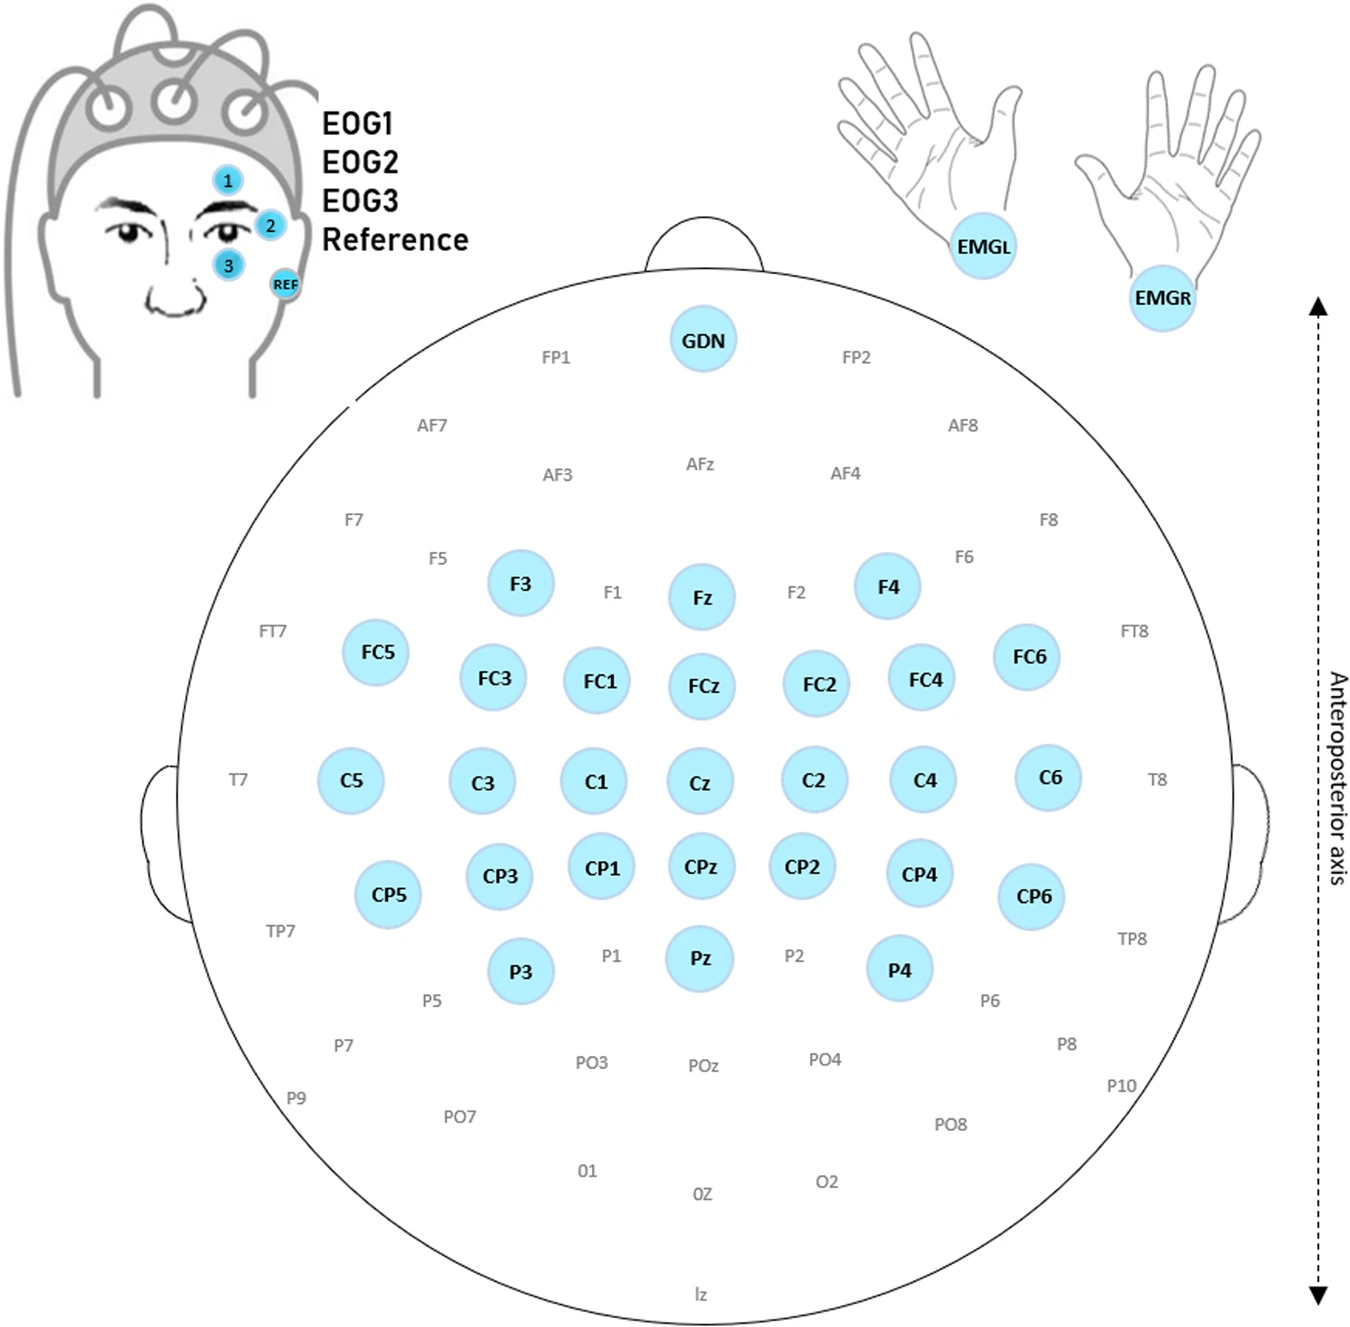
\includegraphics[scale=.2]{./Figures/EEG-10-20.jpg}
	\caption{Imagen tomada de la página oficial del procesador\protect\footnotemark.}
	\label{fig:electrodos}	
\end{figure}


% El conjunto de datos final se estructuró en registros correspondientes a 60 participantes sanos. Gracias a la integración con la biblioteca MOABB, se logró una segmentación uniforme de los ensayos, permitiendo que cada archivo incluyera las etiquetas de clase para la mano izquierda y la mano derecha de manera consistente. Esta organización facilitó el tratamiento digital de la información en la infraestructura en la nube, asegurando la integridad de las señales antes del proceso de entrenamiento de los modelos.

En la tabla \ref{tab:dataset-dreyer} se presentan las especificaciones técnicas que caracterizan al conjunto de datos utilizado en este trabajo, se destaca la cantidad de participantes, la duración de cada ensayo, el número de ensayos por clase y la calidad de las señales obtenidas. Esta información es crucial para comprender el contexto en el que se desarrolló el modelo de clasificación de imaginación motriz y para evaluar su desempeño en función de las características del conjunto de datos.

\begin{table}[h]
	\centering
	\caption[dataset dreyer]{Especificaciones técnicas del conjunto de datos Dreyer2023A.}
	\begin{tabular}{L{8cm} L{4cm}}
		\toprule
		\textbf{Parámetro} & \textbf{Valor} \\
		\midrule
		Número de sujetos           	& 60 \\
		Número de canales EEG        & 27 \\
		Número de clases de imaginación motriz 	& 2 (mano izquierda, mano derecha) \\
		Frecuencia de muestreo  		& 500 Hz \\
		Duración de ensayo  		    & 5 s \\
		Runs por sujeto				& 6 \\
		Ensayos por clase por sujeto & 20 \\
		\bottomrule
	\end{tabular}
	\label{tab:dataset-dreyer}
\end{table}

\section{Métodos tradicionales para EEG y extracción automática de características}
Tradicionalmente, la decodificación de la imaginación motriz se fundamenta en el uso de algoritmos de aprendizaje automático o Machine Learning combinados con una etapa crítica de ingeniería de rasgos manual.

El método tradicional generalizado consiste en la aplicación de CSP. Esta técnica se basa en la descomposición de las señales para maximizar la varianza entre clases, que facilita la separación de los estados mentales de movimiento \cite{riascos2024machine}. Tras la extracción de estos patrones, se emplean clasificadores de baja complejidad como el análisis discriminante lineal o LDA (del inglés, \textit{Linear Discriminant Analysis}) y las máquinas de vectores de soporte o SVM (del inglés, \textit{Support Vector Machines}). Si bien estos métodos demuestran eficacia en entornos controlados, presentan una alta sensibilidad a la colocación de los electrodos y requieren un ajuste experto de las bandas de frecuencia para cada sujeto.

Frente a estas limitaciones, el avance hacia el aprendizaje profundo o \textit{Deep Learning} ha permitido el desarrollo de modelos capaces de realizar la extracción automática de características. A diferencia de los esquemas clásicos, estas arquitecturas aprenden representaciones jerárquicas directamente a partir de los datos crudos, se reduce la necesidad de una ingeniería de rasgos manual.

Sin embargo, diversos estudios han señalado que la calidad de la adquisición de las señales EEG continúa siendo un factor determinante en el desempeño de estos modelos. Una configuración deficiente en la toma de muestras o una inadecuada colocación de los sensores puede introducir artefactos que las redes neuronales interpretan erróneamente como patrones fisiológicos, que afecta la robustez de la predicción. Por lo tanto, aunque los modelos de aprendizaje profundo contengan la capacidad de identificar características complejas, su desempeño depende en gran medida de la calidad y fidelidad de las señales de entrada.


En la tabla \ref{tab:comparacionmetodos} se presenta una comparación entre los métodos tradicionales de procesamiento de EEG y las técnicas de aprendizaje profundo. Estas destacan sus características, ventajas y limitaciones en el contexto del análisis de señales EEG para la clasificación de tareas de imaginación motriz.

\begin{table}[H]
	\centering
	\caption[Comparación entre modelos]{Comparación entre métodos tradicionales y modelos de aprendizaje profundo para el análisis de EEG.}
	\begin{tabular}{L{3cm} L{4cm} L{4cm}}
		\toprule
		\textbf{Característica} & \textbf{Métodos Tradicionales (CSP, SVM, LDA)} & \textbf{Aprendizaje Profundo (CNN, EEGNet)} \\
		\midrule
		Extracción de rasgos & Manual y basada en conocimiento experto. & Automática a partir de los datos de entrada. \\
		Sensibilidad al ruido & Muy alta, requiere filtros manuales estrictos. & Moderada, depende de la calidad del dato. \\
		Manejo de datos & Requiere segmentación y filtrado previo. & Procesamiento con preprocesamiento mínimo. \\
		Rendimiento & Limitado ante señales no estacionarias. & Mayor robustez y escalabilidad. \\
		Dependencia & Alta dependencia de calibración por sujeto. & Posibilidad de aprendizaje transferido. \\
		\bottomrule
	\end{tabular}
	\label{tab:comparacionmetodos}
\end{table}

\section{Arquitecturas de redes neuronales para EEG en imaginación motriz}

Las CNN se consolidan como una de las herramientas más eficaces para la extracción de características. Mediante el uso de filtros de convolución, estas redes permiten identificar patrones de activación en regiones específicas de la corteza motora, que simula de manera automática el comportamiento de los filtros espaciales tradicionales. Por ello, El uso de las CNN facilita la detección de cambios en la amplitud de los ritmos sensorimotores asociados a la intención de movimiento de las extremidades. 

Por otro lado, para el análisis de la dinámica temporal de las señales EEG, las redes neuronales recurrentes o RNN (del inglés, \textit{Recurrent Neural Networks}), específicamente las unidades de memoria de largo corto plazo o LSTM (del inglés, \textit{Long Short-Term Memory}) y las unidades recurrentes calificadas o GRU (del inglés, \textit{Gated Recurrent Units}) permiten modelar la evolución de la señal a lo largo del tiempo, estas utilizan mecanismos de puertas para retener información relevante y descartar el ruido transitorio. Mientras que las LSTM emplean una estructura compleja para gestionar la memoria a largo plazo, las GRU ofrecen una alternativa más eficiente en términos computacionales, que mantienen un rendimiento competitivo en la clasificación de series temporales de EEG.


Por último, los enfoques híbridos han sido ampliamente utilizados para integrar las ventajas de distintos modelos en el análisis de señales EEG. En particular, las arquitecturas de tipo CNN-LSTM combinan la capacidad de las redes convolucionales para extraer características espaciales con la habilidad de las redes recurrentes para modelar dependencias temporales \cite{zhang2021eeg}.

En este tipo de arquitecturas, las capas convolucionales permiten identificar patrones relevantes en la distribución espacial de los electrodos, mientras que las capas recurrentes procesan la evolución temporal de dichas características. Esta combinación resulta adecuada para el manejo de la alta dimensionalidad de las señales EEG, que facilita la construcción de representaciones robustas previas a la etapa de clasificación.


El enfoque híbrido y las arquitecturas de redes neuronales aplicadas al análisis de señales EEG, se puede observar en la figura \ref{fig:arquitecturas}, donde se ilustra la estructura general de cada modelo y su aplicación específica en el contexto de la clasificación de tareas de imaginación motriz, se destacan las capas de procesamiento y la forma en que cada arquitectura aborda la extracción de características espaciales y temporales para mejorar la precisión de la predicción de la intención motora a partir de señales EEG.

\begin{figure}[htpb]
	\centering
	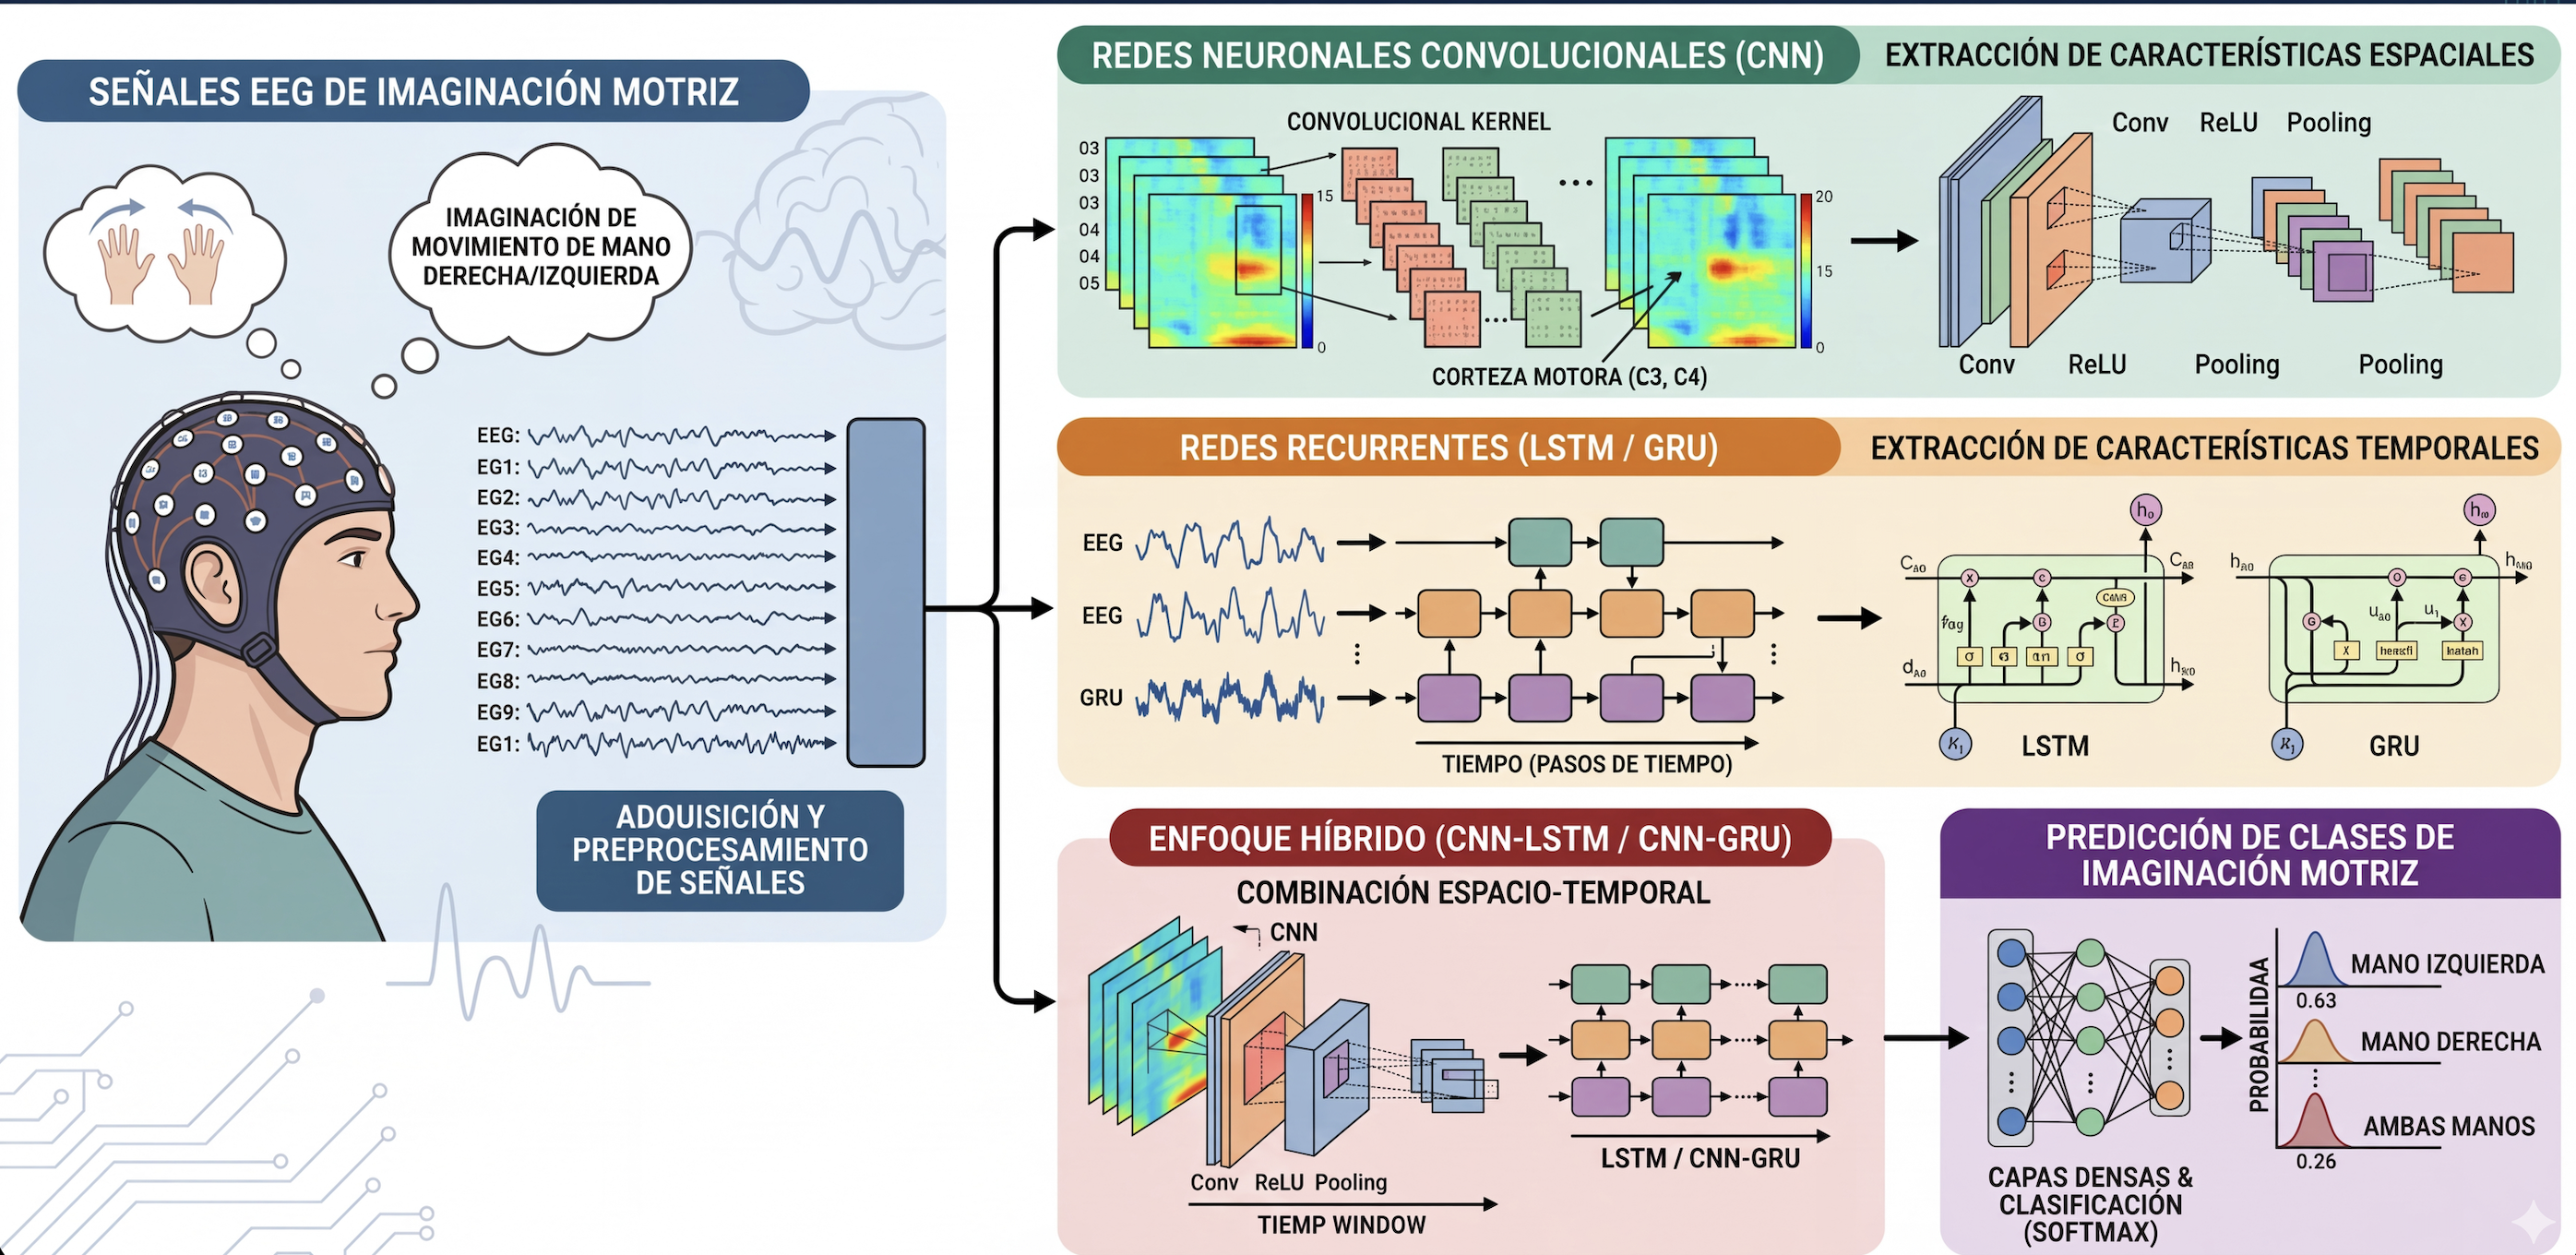
\includegraphics[scale=.26]{./Figures/redes-neuronales-eeg.png}
	\caption{Estructura general de los modelos y su aplicación en la clasificación
de tareas de imaginación motriz.}
	\label{fig:arquitecturas}	
\end{figure}


En la tabla \ref{tab:comparacionarquitecturas} se presenta una comparación técnica entre las arquitecturas de redes neuronales aplicadas al análisis de señales EEG, se destaca las características, ventajas y limitaciones en el contexto de la clasificación de tareas de imaginación motriz. Esta comparación proporciona una visión integral de cómo cada enfoque contribuye al procesamiento de las señales EEG y a la mejora del rendimiento en la decodificación de la intención motora.
\begin{table}[h]
	\centering
	\caption[Comparación entre arquitecturas]{Comparación entre arquitecturas CNN, LSTM y CNN-LSTM aplicadas al análisis de señales EEG.}
	\begin{tabular}{L{2.5cm} L{3.5cm} L{3.5cm} L{3.5cm}}
		\toprule
		\textbf{Característica} & \textbf{CNN} & \textbf{LSTM / GRU} & \textbf{CNN-LSTM} \\
		\midrule
		Tipo de procesamiento 
		& Espacial (filtros convolucionales)
		& Temporal (modelado secuencial) 
		& Espacial + temporal combinado \\

		Extracción de características 
		& Automática en dominios espaciales locales 
		& Basada en dependencias temporales 
		& Extracción jerárquica espacio-temporal \\\\

		Manejo de dependencias temporales 
		& Limitado 
		& Alto (memoria de corto y largo plazo) 
		& Alto (integrado con características espaciales) \\\\

		Complejidad computacional 
		& Moderada 
		& Alta 
		& Alta \\

		Robustez frente a ruido 
		& Moderada 
		& Moderada 
		& Alta (por integración de representaciones) \\\\

		Ventaja principal 
		& Detección de patrones espaciales en electrodos 
		& Modelado de dinámica temporal de la señal 
		& Captura conjunta de patrones espaciales y temporales \\\\

		Limitación principal 
		& No modela secuencias largas 
		& Alto costo y entrenamiento más complejo 
		& Mayor complejidad y necesidad de ajuste fino \\

		Aplicación en EEG 
		& Identificación de activación cortical localizada 
		& Análisis de evolución temporal de ritmos cerebrales 
		& Clasificación integral de tareas de imaginación motriz \\

		\bottomrule
	\end{tabular}
	\label{tab:comparacionarquitecturas}
\end{table}
\footnotetext{Imagen generada por inteligencia artificial.}

\chapter{Diseño e implementación} % Main chapter title

\label{Chapter3} % Change X to a consecutive number; for referencing this chapter elsewhere, use \ref{ChapterX}

En este capítulo se describen las etapas de diseño y el ajuste del sistema orientado a la clasificación de tareas de imaginación motriz. En las siguientes secciones se detallan la arquitectura del sistema, el tratamiento de los datos de origen, el desarrollo y entrenamiento de los modelos de aprendizaje profundo, así como el protocolo de evaluación y el despliegue final en la infraestructura de la nube.

%----------------------------------------------------------------------------------------
%	SECTION 1
%----------------------------------------------------------------------------------------
\section{Arquitectura del sistema}

En esta sección se describe la arquitectura general del sistema que se utilizó para la predicción de tareas de imaginación motriz a partir de EEG.

El sistema se estructuró como un flujo secuencial compuesto por etapas de preparación de datos, preprocesamiento, extracción de características, inferencia mediante modelos de aprendizaje profundo y despliegue en infraestructura cloud. Este enfoque permitió integrar el procesamiento de señales EEG con servicios distribuidos, facilitando la escalabilidad y la eficiencia en la ejecución de los modelos.

La fuente de datos correspondió al conjunto de datos Dreyer2023A \cite{dreyer2023large}. Este contiene registros de señales EEG asociados a tareas de imaginación motriz. Dicho conjunto fue utilizado como base para el entrenamiento y evaluación de los modelos, sin realizar procesos de adquisición directa de señales.

Luego, se implementó una etapa de preprocesamiento orientada a mejorar la relación entre la señal y el ruido. En esta fase se aplicaron técnicas de filtrado y segmentación, con el fin de aislar ventanas relevantes para el análisis. Este procedimiento permitió reducir la variabilidad inherente a las señales EEG y facilitar el aprendizaje de patrones discriminativos.

La extracción de características se abordó mediante arquitecturas de redes neuronales, que permitieron modelar dependencias espaciales y temporales presentes en las señales. Se consideraron enfoques híbridos capaces de capturar correlaciones entre canales y dinámicas temporales, lo que resulta fundamental en tareas de imaginación motriz \cite{zhang2021eeg}.

El módulo de inferencia se diseñó para recibir las representaciones procesadas y generar una predicción de la tarea imaginada. Este módulo se integró con un servicio web, que permitió exponer la funcionalidad del modelo por medio de una API RESTful. De esta manera, se facilitaría la interacción con aplicaciones externas y la posibilidad de realizar predicciones en tiempo real.

A continuación, se presenta la arquitectura general del sistema propuesto en la figura \ref{fig:cloud-arquitecturas}, en la que se ilustran las etapas principales del flujo de procesamiento y su integración dentro del entorno cloud.
\begin{figure}[h!]
    \centering
    % Use width=\textwidth or a fraction to fit without stretching
	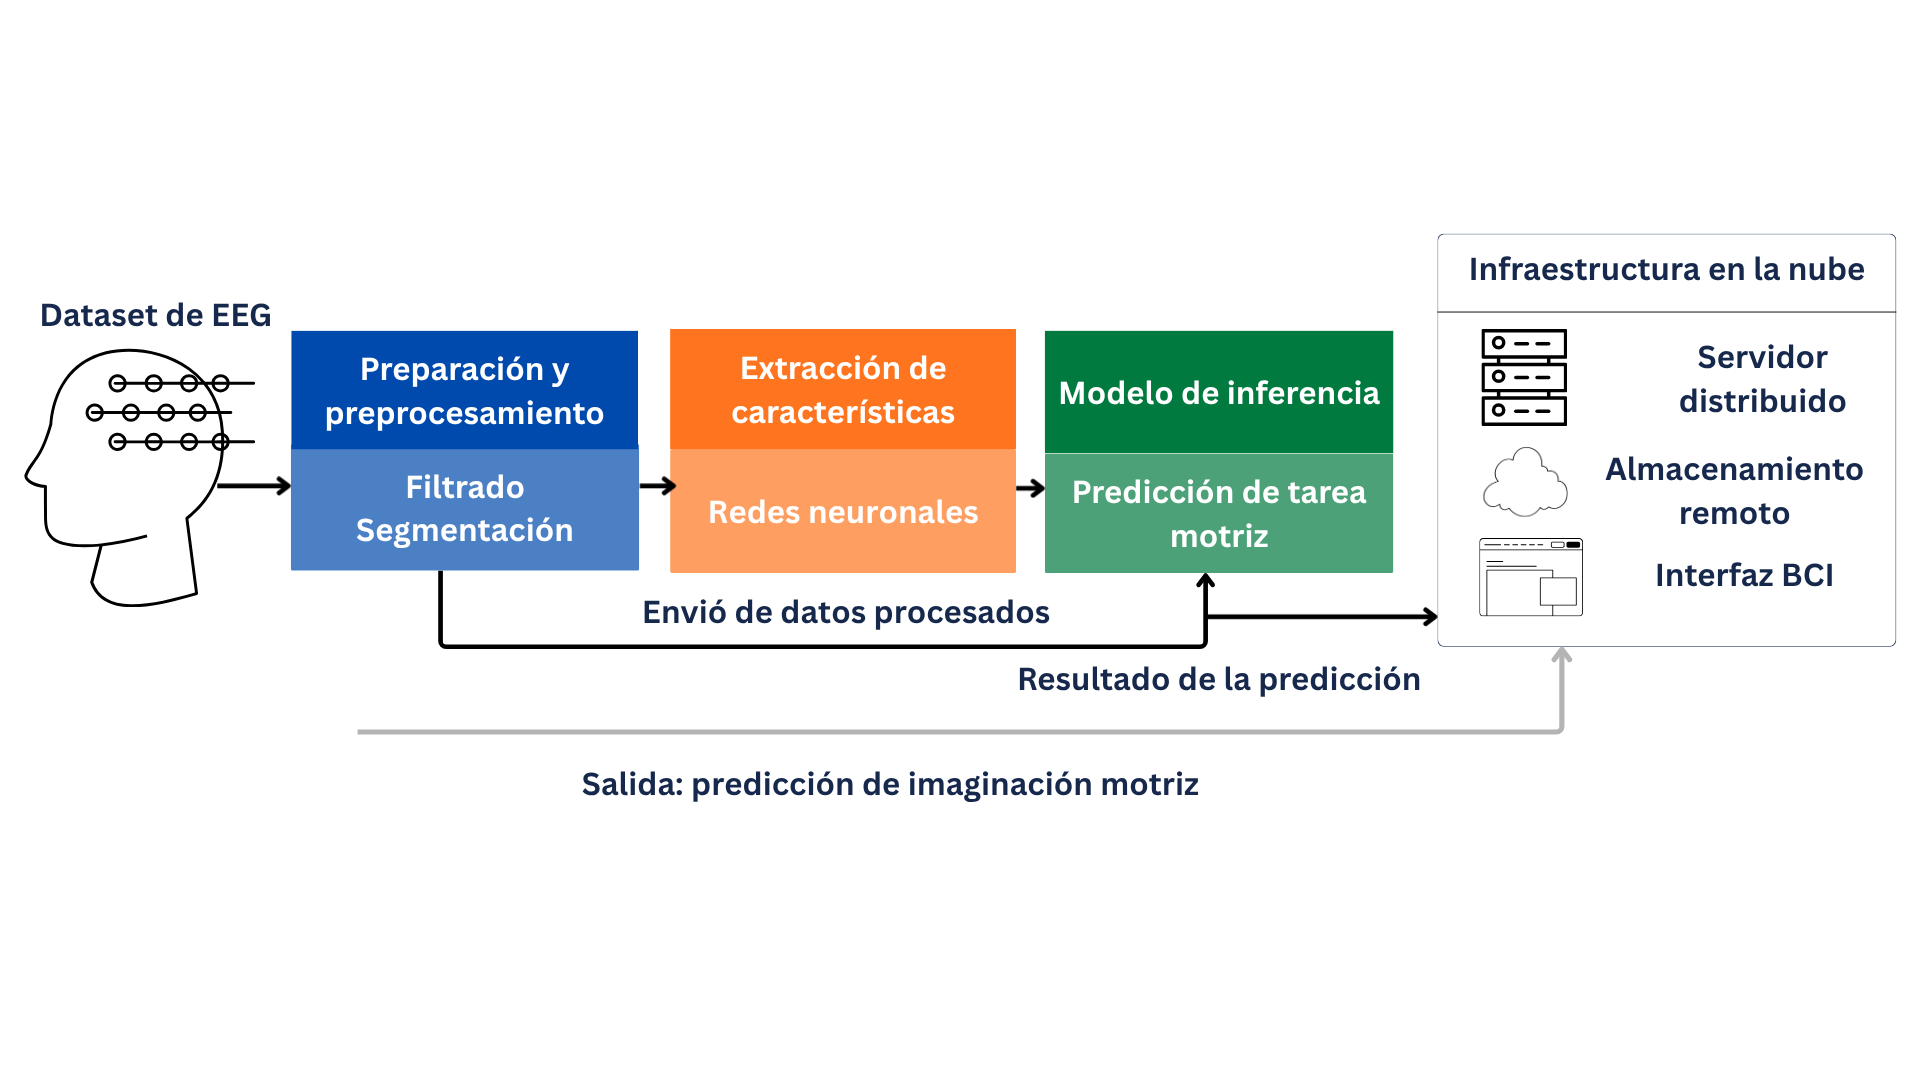
\includegraphics[width=\linewidth]{./Figures/arquitectura-interfaz-cerebro-v2.png}
    % \includegraphics[width=0.8\textwidth]{image_name.pdf} 
    \caption{Diagrama de la arquitectura general del sistema.}
	\label{fig:cloud-arquitecturas}
\end{figure}


Finalmente, el sistema se desplegó bajo un paradigma cloud, que permitió desacoplar el procesamiento intensivo del entorno local. Esta arquitectura facilitó la implementación de una interfaz cerebro-computador cloud, en la que las señales fueron procesadas de manera remota para la generación de resultados.

La arquitectura descrita estableció un flujo completo desde la preparación de los datos hasta la obtención de predicciones, garantizando modularidad, escalabilidad y capacidad de integración con aplicaciones externas.

%----------------------------------------------------------------------------------------
%	SECTION 2
%----------------------------------------------------------------------------------------


\section{Preparación y preprocesamiento de los datos}

En esta sección se describen los métodos aplicados a las señales EEG antes del entrenamiento de los modelos, incluyendo las etapas de preparación, preprocesamiento, filtrado, segmentación, transformación y estandarización de los datos.

\subsection{Preparación de los datos}

En la etapa de preparación, se realizó la carga de los registros EEG considerando su organización estructurada por sujetos, sesiones y ensayos, conforme a la definición del conjunto de datos Dreyer2023A descrito en \cite{dreyer2023large}. Este conjunto incluye múltiples participantes sometidos a experimentos de imaginación motriz de mano izquierda y derecha, con un número significativo de ensayos por sesión, lo que permitió disponer de un volumen amplio de datos para el entrenamiento de los modelos . Por medio de la interfaz de MOABB (del inglés, \textit{Mother Of All BCI Benchmarks}), se accedió a los datos en un formato estandarizado basado en eventos, lo que facilitó la manipulación de las señales y su integración en el flujo de procesamiento.

Después, se identificaron los eventos asociados a cada tarea de imaginación motriz, que correspondían a etiquetas discretas como mano izquierda y mano derecha dentro del paradigma de clasificación binaria . Estos eventos permitieron segmentar las señales continuas en ensayos individuales alineados temporalmente con los estímulos experimentales. Cada ensayo representó una instancia etiquetada del conjunto de datos, lo que permitió estructurar la información en un esquema supervisado ideal para el entrenamiento de los modelos.

Por otra parte, se consideró la consistencia en la organización de los canales EEG y la sincronización temporal de las señales, garantizando que cada muestra mantuviera la correspondencia entre dimensiones espaciales y temporales. Este proceso permitió transformar los datos originales en una representación homogénea, facilitando su posterior procesamiento y asegurando la compatibilidad en terminos de entradas estructuradas y uniformes con los modelos.

\subsection{Preprocesamiento de los datos}

En la fase de preprocesamiento, se aplicó un filtrado de las señales EEG con el objetivo de mejorar la relación señal y ruido para resaltar los componentes relevantes para la tarea de clasificación. Para eso, se empleó un filtro pasa banda en el rango de 8 a 30 Hz, se considera que este intervalo abarca las bandas $\mu$ (aproximadamente 8–13 Hz) y $\beta$ (13–30 Hz), que están estrechamente relacionadas con la actividad cortical asociada a la imaginación motriz \cite{pfurtscheller2001motor, zhang2021eeg}. Estas bandas presentan patrones característicos de desincronización y sincronización relacionados con la ejecución o imaginación de movimientos, lo que las convierte en una fuente relevante de información discriminativa.

El filtrado permitió atenuar componentes de muy baja frecuencia, asociadas a derivas de la señal y artefactos fisiológicos como la actividad electrodermal, así como reducir el ruido de alta frecuencia proveniente de interferencias externas o actividad muscular no deseada. De esta manera, se preservó la información espectral de interés mientras se eliminaban componentes irrelevantes para la tarea.

De igual forma, este proceso contribuyó a estabilizar la señal y a reducir la variabilidad no deseada entre ensayos, que facilitó la posterior etapa de segmentación y el aprendizaje de patrones por parte de los modelos. El filtrado aplicado se mantuvo consistente para todos los sujetos y sesiones, además, se garantizó uniformidad en el tratamiento de los datos y se evitó posibles sesgos introducidos por diferencias en el preprocesamiento. 

\subsection{Segmentación de los datos}

En la fase de segmentación, se realizó la segmentación temporal de las señales EEG en ventanas alineadas con los eventos de estímulo, con el fin de aislar los intervalos de interés asociados a cada tarea de imaginación motriz. A partir de los registros continuos, se extrajeron segmentos (epochs) definidos en un intervalo temporal específico posterior a la aparición del estímulo, asegurando que cada ventana contuviera la respuesta cerebral relevante para la tarea. Este procedimiento permitió sincronizar las señales en relación con el inicio del evento, garantizando coherencia temporal entre las muestras.

Cada segmento fue definido con una duración fija, que permitió obtener representaciones homogéneas en términos de longitud temporal. Esta procedimiento resultó muy útil para su posterior utilización en los modelos, que requieren entradas con dimensiones consistentes. De igual forma, se evitó la inclusión de intervalos previos al estímulo que no aportaran información discriminativa, enfocando el análisis en las regiones temporales donde se manifiestan patrones asociados a la imaginación motriz.

La segmentación generó múltiples muestras independientes a partir de cada registro continuo, se incrementó el número de ejemplos disponibles para el entrenamiento. Este incremento en la cantidad de datos permitió mejorar la capacidad de generalización de los modelos, al exponerlos a una mayor variabilidad intra e intersujeto.

Adicionalmente, se mantuvo la correspondencia entre cada segmento y su respectiva etiqueta de clase, preservando la integridad del conjunto de datos supervisado. Este proceso permitió transformar las señales EEG continuas en un conjunto estructurado de muestras etiquetadas, adecuado para su utilización en tareas de clasificación.

En la tabla \ref{tab:preprocesamiento-data}, se presentan los parámetros utilizados durante las etapas de preparación y preprocesamiento de las señales EEG.

\begin{table}[h]
\centering
\caption[Parámetros Dataset]{Parámetros de preparación y preprocesamiento de \mbox{señales} EEG}
\label{tab:preprocesamiento-data}
\begin{tabular}{|l|l|l|}
\hline
\textbf{Etapa} & \textbf{Parámetro} & \textbf{Valor} \\ \hline

\multirow{10}{*}{Preparación} 
& Dataset & Dreyer2023  \\ \cline{2-3}
& Acceso a datos & MOABB  \\ \cline{2-3}
& Número de sujetos & 60 \\ \cline{2-3}
& Tipo de tarea & Imaginación motriz \\ \cline{2-3}
& Clases & Mano izquierda / Mano derecha \\ \cline{2-3}
& Número de canales EEG & 27 \\ \cline{2-3}
& Sistema de electrodos & 10-20 \\ \cline{2-3}
& Frecuencia de muestreo & 512 Hz \\ \cline{2-3}
& Número de runs por sesión & 6 \\ \cline{2-3}
& Ensayos por run & 40 \\ \hline

\multirow{4}{*}{Preprocesamiento}
& Tipo de señal & Señales crudas \\ \cline{2-3}
& Filtro aplicado & Pasa banda \\ \cline{2-3}
& Rango de filtrado & 8--30 Hz \\ \cline{2-3}
& Bandas analizadas & $\mu$ (8--13 Hz), $\beta$ (13--30 Hz) \\ \hline

\multirow{3}{*}{Segmentación}
& Tipo de ventana & Epochs alineados a estímulo \\ \cline{2-3}
& Intervalo temporal & Posterior al estímulo \\ \cline{2-3}
& Duración de ventana & Fija \\ \hline

Normalización & Tipo & Estandarización por muestra \\ \hline

Estructuración & Formato de entrada & (canales $\times$ tiempo) \\ \hline

\end{tabular}
\end{table}
% Chapter 4

\chapter{Ensayos y resultados} % Main chapter title

\label{Chapter4} % For referencing this chapter elsewhere, use \ref{Chapter4}

En este capítulo se presentan los ensayos realizados para evaluar el desempeño del sistema de clasificación de tareas de imaginación motriz. Se describe el protocolo experimental aplicado, el desempeño alcanzado por las arquitecturas implementadas, la capacidad predictiva del sistema y la comparación con enfoques tradicionales, junto con el análisis de los resultados obtenidos.

%----------------------------------------------------------------------------------------
%	SECTION 1
%----------------------------------------------------------------------------------------

\section{Ensayos de modelos}
\label{sec:ensayosModelos}

Para el desarrollo de los ensayos se estableció un protocolo experimental orientado a evaluar el comportamiento de las tres arquitecturas implementadas sobre el conjunto Dreyer2023A. El protocolo definió de manera explícita la partición de los datos, la estrategia de evaluación, la configuración de los experimentos y el número de ejecuciones, con el fin de garantizar condiciones comparables entre los modelos y la reproducibilidad de los resultados.

La partición del conjunto de datos se realizó considerando la organización del conjunto por sujetos. Se asignaron cuarenta y dos sujetos al conjunto de entrenamiento y los dieciocho restantes al conjunto de validación, lo que correspondió a una proporción de setenta por ciento y treinta por ciento, respectivamente. Esta división garantizó que los modelos no observaran durante el entrenamiento las señales de los sujetos empleados para su evaluación, de modo que las métricas obtenidas reflejaron la capacidad de generalización frente a usuarios no vistos. La asignación de sujetos a cada conjunto se mantuvo fija en todas las ejecuciones, lo que permitió comparar el desempeño de las arquitecturas sobre los mismos datos de validación.

La estrategia de evaluación consistió en entrenar cada arquitectura sobre el conjunto de entrenamiento y cuantificar su desempeño sobre el conjunto de validación. Para cada muestra, el modelo generó un puntaje de pertenencia a las clases de imaginación motriz que se comparó con un umbral de decisión. A partir de los aciertos y errores desagregados por clase, se calcularon las métricas de exactitud, precisión, exhaustividad y puntuación F1, cuya definición se presentó en el protocolo de evaluación del capítulo anterior.

La configuración estructural de cada arquitectura se obtuvo mediante el proceso de búsqueda de hiperparámetros descrito en el capítulo anterior. El entorno de optimización ejecutó cincuenta ensayos por arquitectura, explorando los rangos definidos para la tasa de aprendizaje, el tamaño del lote, el dropout y los parámetros estructurales específicos de cada modelo. La configuración que reportó el mayor desempeño en el conjunto de validación durante la búsqueda fue la adoptada para los ensayos definitivos.

Con el fin de cuantificar la estabilidad del desempeño, cada arquitectura se entrenó y evaluó en diez ejecuciones independientes. Las ejecuciones difirieron únicamente en la inicialización aleatoria de los pesos y en la selección de los lotes de entrenamiento, manteniéndose idénticas la partición de los datos y la configuración de hiperparámetros. Para cada métrica se calculó el promedio y la desviación sobre las diez ejecuciones, de modo que los resultados presentados en las secciones siguientes reflejaron tanto el valor esperado del desempeño como su variabilidad.

En la tabla \ref{tab:config_experimentos} se resume la configuración de los experimentos realizados.

\begin{table}[htbp]
\centering
\caption{Configuración de los experimentos realizados.}
\label{tab:config_experimentos}

\begin{tabular}{L{6cm}L{6cm}}
\toprule
\textbf{Aspecto} & \textbf{Configuración} \\
\midrule

Conjunto de datos &
Dreyer2023A \\ 

Sujetos de entrenamiento &
42 (70 \%) \\ 

Sujetos de validación &
18 (30 \%) \\ 

Arquitecturas evaluadas &
CNN, RNN-LSTM y CNN-LSTM \\ 

Ensayos de optimización &
50 por arquitectura \\ 

Ejecuciones independientes &
10 por arquitectura \\ 

Métricas de desempeño &
Exactitud, precisión, exhaustividad y F1 \\ 

\end{tabular}
\end{table}

\FloatBarrier

%----------------------------------------------------------------------------------------
%	SECTION 2 (pendiente)
%----------------------------------------------------------------------------------------

% \section{Desempeño del modelo}
\include{Chapters/Chapter5}

%----------------------------------------------------------------------------------------
% Apéndices
%----------------------------------------------------------------------------------------

\appendix

% Incluir apéndices desde archivos separados si es necesario
%\include{Appendices/AppendixA}

%----------------------------------------------------------------------------------------
% Bibliografía
%----------------------------------------------------------------------------------------

\renewcommand{\bibname}{Bibliografía} % Para asegurarte de que el título sea correcto
\phantomsection % Necesario para que el enlace del marcador sea correcto

\printbibliography[heading=bibintoc]

\end{document}






